The following section deals with the training process of YOLO and MobileNetV2-UNet.
For both networks similar experiments were performed each sub-experiment was repeated three times each with a different seed.
The used seeds were: $\{42, 1337, 0xDEADBEEF\}$

First an initial learning rate search was performed, here six to seven learning rates were tested on the basic dataset.
The basic dataset is the default train/valid/test split (table \ref{tab:data_distribution} and \ref{tab:yolo_classes}) without any pre-augmentations of the training set.
The best performing learning rate is then taken as the baseline for the following experiments.

The second conducted experiment is a search for the perfect configuration of so called offline augmentations.
Offline augmentations are a 90\textdegree, 180\textdegree and a 270\textdegree  rotation of the original image, as well as a horizontal flip and again three rotations of the flipped image.
Furthermore, as has been described in section \ref{sec:data}, for some images a mask has been created, which is projected on different checkered background images to increase the amount of those.
This offline augmentation is referred to as projection.
The search for the best configuration is performed by taking all possible configuration of those three offline augmentations.

Afterwards, an ablation study is performed for various augmentations, with different parameters.
The augmentations in that study are also referred to as online augmentations, since they are performed at training time.
The occurrence probability of those augmentations is set to 50\%.
Since, the augmentations slightly differ for each network they are explained in the respective subsection.

The last experiment step is formed by a fine tuning step, where a grid search was performed.
The grid search always utilizes the best performing offline and online augmentations and consists of various learning rates, batch sizes and other network specific parameters.

The evaluation of each experiment is done by comparing the mean and standard deviation of each experiment, if the mean is higher, in almost all cases this configuration is considered to be superior to another one, the standard deviation should still remain in a reasonable area.

\subsection{YOLOv4-Tiny}

To perform any experiments with \ac{YOLO} first an initial configuration was defined.
This configuration is given in \ref{tab:initial_yolo_config}, it consist of a fixed batch size of $64$, the \ac{CIoU} loss as described in section \ref{sec:yolo}. \ac{SGD} with momentum was used as the optimizer with a momentum rate of $0.9$.

\begin{table}[H]
\footnotesize
\begin{center}
\begin{tabular}{|l|l|}

\hline
\textbf{Batch Size} & $64$\\
\hline
\textbf{Loss} & CIoU \\
\hline
\textbf{Optimizer} & \ac{SGD} with Momentum ($\mu = 0.9$)\\
\hline
\textbf{Burn in} & 1000 steps \\
\hline
\textbf{Dataset} & No pre-augmentation performed \\
\hline

\end{tabular}
\caption{The initial training configuration for the experiments performed with the YOLO network.}
\label{tab:initial_yolo_config}
\end{center}
\end{table}

Redmon et al. have pointed out that training \ac{YOLO} is unstable, when the full learning rate is applied without proper scheduling \cite{yolov2}.
This was also tested in this thesis and can be confirmed, all learning rates which were tested in the initial learning rate search diverged when used without a scheduling mechanism.
The proposed scheduling function by Redmon et al., which is still used in the current \ac{YOLOv4} \cite{yolov4}, is given by the following formula:

\begin{equation}
    lr(step) =
    \begin{cases}
        lr_{base} * (\frac{step}{burn\_in})^4 & \textbf{if } step < burn\_in\\
        lr_{base}                             & \textbf{else}
    \end{cases}
\end{equation}

Where a step is defined as one whole batch and the $burn\_in$ is set to $1000$ steps.

All trained experiments were optimized for a slightly changed COCO mAP metric.
COCO uses a $mAP0.5:0.95:0.05$, while in this thesis $mAP0.5:0.75:0.05$ is used, since an \ac{IoU} of $0.75$ is considered to be enough for the whole system to work properly in most circumstances.
All experiments are optimized for this metric, which means that at every step the mAP is calculated for the whole validation set and if the mAP is better than the previously calculated mAP, the weights of the network are stored and used for further evaluation.

\subsubsection{Experiment: Initial Learning Rate Search}

The first experiment was executed to find an initial learning rate for further experiments.
The parameters for the network were set to the ones in table \ref{tab:initial_yolo_config} and kept for all training runs.
The results of the training runs can be found in figure \ref{fig:yolo_lr_experiment_results}, where the mean of mAP for the three performed runs is shown for each learning rate.
The full results of the learning rate search with classwise performance can be found in table \ref{tab:yolo_init_lr_results} in the appendix.
It can be observed that the learning rate $0.001$ has the highest \ac{mAP}, therefore it is selected as the default learning rate for further experiments.
This experiment has shown that the text class and especially the arrow classes showed consistently bad performance over all learning rates.

\begin{figure}
\begin{center}
    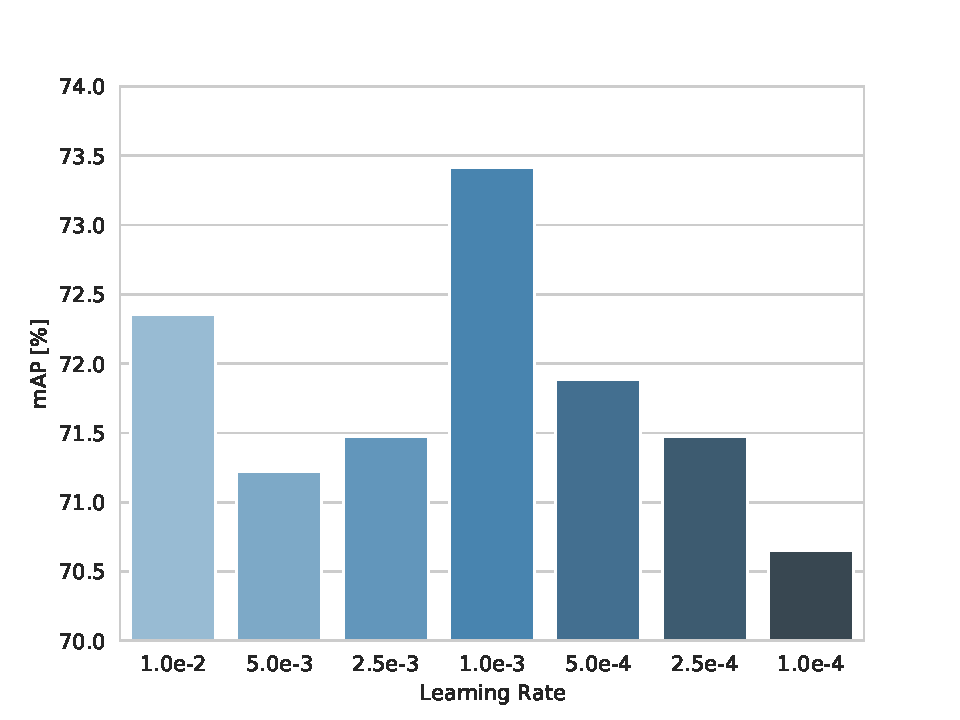
\includegraphics[width=13cm]{imgs/yolo_lr_experiment.pdf}
    \caption{The results of the initial learning rate search shown on the validation set, as the mean of the mAPs of three separate training runs.}
    \label{fig:yolo_lr_experiment_results}
\end{center}
\end{figure}


\subsubsection{Experiment: Offline Augmentations}

This experiment was conducted to find the optimal configuration of offline augmentations, where the offline augmentations are projection (copy-paste augmentation \cite{copypaste_aug}), three 90\textdegree\ rotations and a horizontal flip.
If both the rotation and the flip augmentation are selected at the same time, then additionally the flipped image is rotated three times.
Again for all runs the YOLO configuration from the previous experiment was used, but additionally now the learning rate is set to the best performing one from the learning rate search experiment.
The new configuration can be found in table \ref{tab:yolo_offline_aug_config}.

\begin{table}[H]
\footnotesize
\begin{center}
\begin{tabular}{|l|l|}

\hline
\textbf{Learning Rate} & $1e^{-3}$ \\
\hline
\textbf{Batch Size} & $64$\\
\hline
\textbf{Loss} & CIoU \\
\hline
\textbf{Optimizer} & SGD with Momentum ($\mu = 0.9$)\\
\hline
\textbf{Burn in} & 1000 steps \\
\hline
\textbf{Dataset} & Pre-augmented with respective experiment configuration \\
\hline

\end{tabular}
\caption{The training configuration for the offline augmentation experiment, where the learning rate is set to the best performing learning rate from the learning rate search and the data is pre-augmented with the respective experiment configuration.}
\label{tab:yolo_offline_aug_config}
\end{center}
\end{table}

The full results with classwise \ac{AP} can be found in the appendix in table \ref{tab:yolo_offline_aug_results}.
\begin{figure}
\begin{center}
    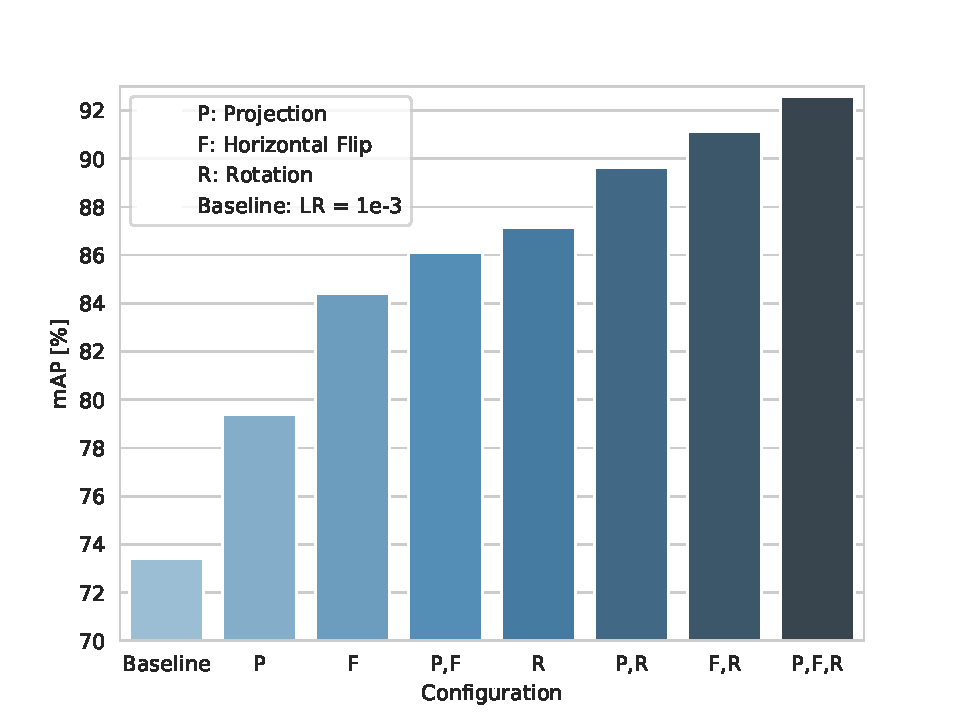
\includegraphics[width=13cm]{imgs/yolo_offline_aug_experiment.pdf}
    \caption{The results of the offline augmentation with the different offline augmentation configurations compared with the results of the best performing learning rate (baseline). When rotation and flip are enabled simultaneously the flipped image also gets rotated three times by 90\textdegree. Results are given as the mean of the mAP of three separate training runs.}
    \label{fig:yolo_offline_aug_results}
\end{center}
\end{figure}

The results for this experiment are also shown in figure \ref{fig:yolo_offline_aug_results}, where a clear trend emerges.
When looking at the results as an ablation it can be seen that each offline augmentation brought an increase in \ac{mAP} and the combination of those too.
Rotation has an absolute increase in mAP, when compared to the baseline (the best performing learning rate), of $13.725\%$, flip shows an increase of $11.000\%$ and the copy-paste augmentation shows an increase of $5.988\%$.
The best configuration is, as expected, the one where all three augmentations are used simultaneously and it has an increase in \ac{mAP} of $19.163\%$.
When specifically comparing the results of the best performing configuration with the baseline, it can be observed that all \ac{ECC} classes have reached a \ac{mAP} greater than $90\%$.
The text and arrow classes have also greatly increased.
Text shows an increase of $24.485\%$ and the mean over the arrow classes shows an increase of $47.988\%$, however those two classes are still not near the desired performance observed at the \acp{ECC}.
It should be pointed out that especially the increase in the text class is very interesting, because this is the only class which is not rotation and flip invariant, i.e. flipping a diode produces again a diode (also for the human perception), but with a different orientation, however flipping a text will produce something no more really interpretable (at least for the human perception).
An explanation why there is still an increase in recognition performance could be that the network starts learning blob like regions, which are located near \acp{ECC}, instead of specific features of the different textual annotations.


\subsubsection{Experiment: Online Augmentations}

The next presented experiment is an ablation study performed on the following augmentations:
\begin{itemize}
    \item Rotation: 10\textdegree, 20\textdegree, 30\textdegree\ (maximum angle to rotate the base image +- value)
    \item Scale: 10\%, 20\%, 30\% (the maximum percentage of the base scale to change +- value)
    \item SafeCrop: 70\%, 80\%, 90\% (the maximum size of the crop relative to the input image size, but considers bounding boxes such that bounding boxes are never cropped)
    \item ColorJitter: 10\%, 20\%, 30\% (the maximum percentage to change the brightness, contrast, saturation or the hue of the input image)
\end{itemize}
These augmentations are performed at runtime and are therefore also referred to as  online augmentations.
Each augmentation was applied with a probability of 50\%.
The general configuration for this experiment is shown in table \ref{tab:yolo_online_config}

\begin{table}[H]
\footnotesize
\begin{center}
\begin{tabular}{|l|l|}

\hline
\textbf{Batch Size} & $64$\\
\hline
\textbf{Loss} & CIoU \\
\hline
\textbf{Optimizer} & SGD with Momentum ($\mu = 0.9$)\\
\hline
\textbf{Burn in} & 1000 steps \\
\hline
\textbf{Dataset} & Pre-augmented with projection, flip and rotation \\
\hline

\end{tabular}
\caption{The YOLO training configuration for the online augmentation experiment. The dataset is now additionally pre-augmented with the projection, flip and rotation augmentation.}
\label{tab:yolo_online_config}
\end{center}
\end{table}

Again, the detailed results can be found in the appendix in the tables \ref{tab:yolo_rotation_augmentation_result}, \ref{tab:yolo_random_scale_augmentation_result}, \ref{tab:yolo_bbox_safe_crop_augmentation_result}, \ref{tab:yolo_color_jitter_augmentation_result}, for each used augmentation separately.
Further, the combined results can be found in figure \ref{fig:yolo_online_aug_results}.
The figure shows, for each augmentation and for all parameters a clear increase.
The best performing parameters are selected and used in the following grid search experiment.

\begin{figure}
\begin{center}
    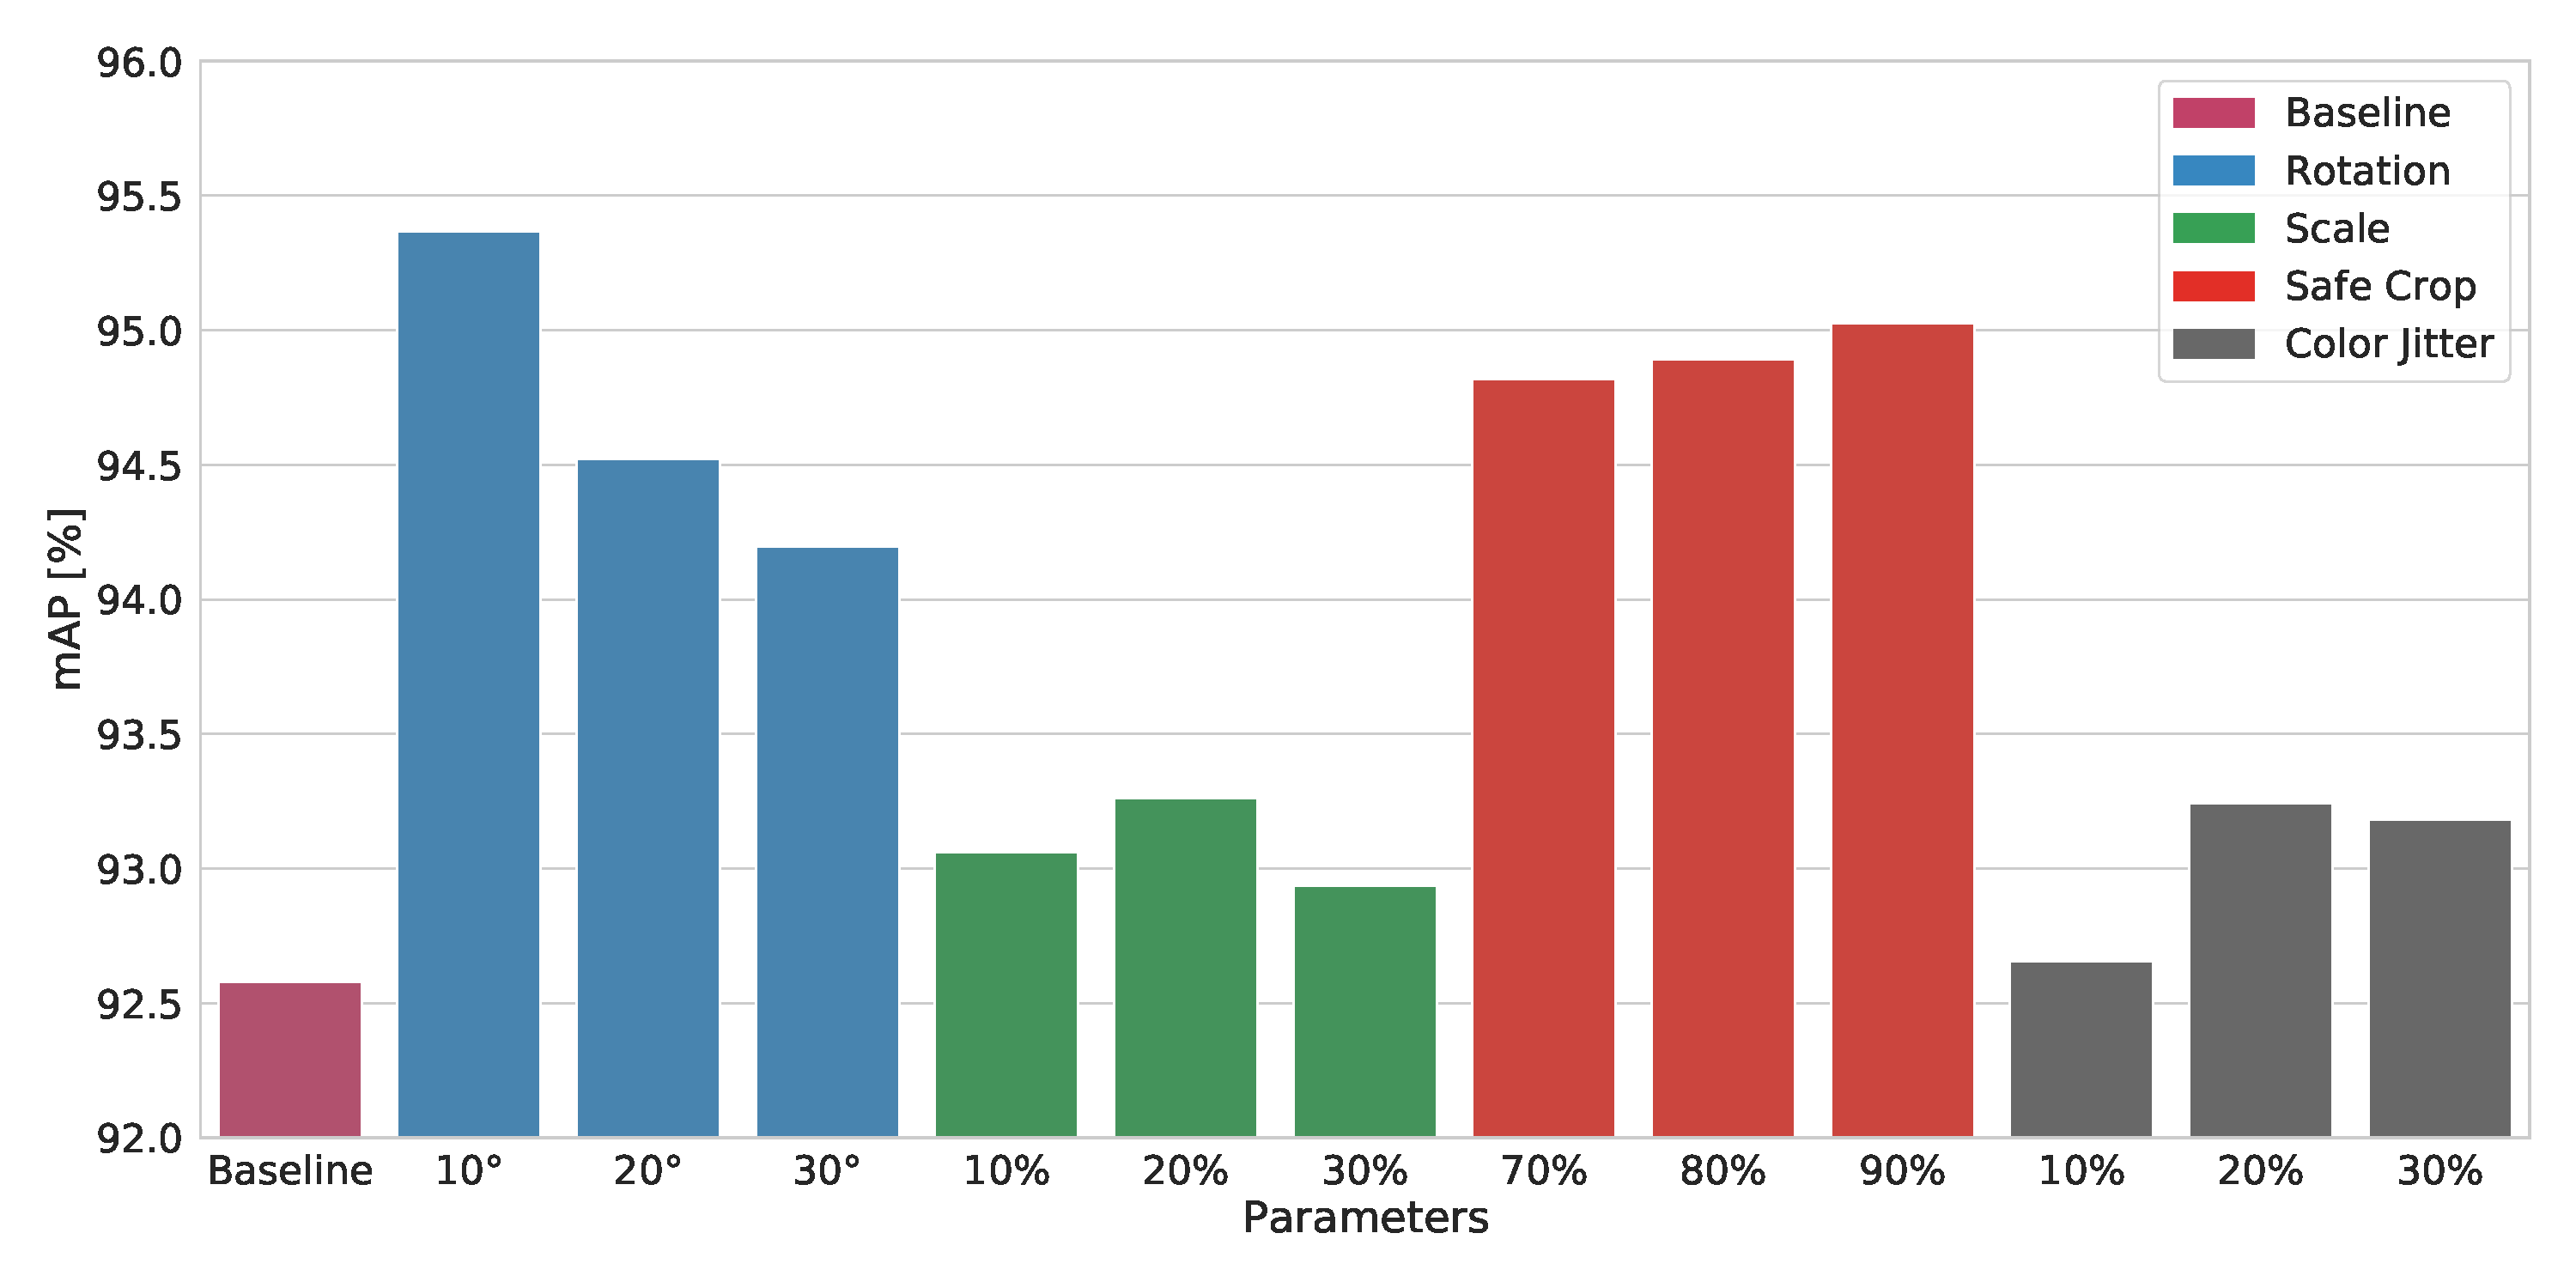
\includegraphics[width=16cm]{imgs/yolo_online_aug_experiment.pdf}
    \caption{Results of the online augmentation experiment compared to the baseline which was established in the offline augmentation experiment. Each augmentation shows a clear increase in mAP in comparison to the baseline. The best performing parameters are used together in the grid search experiments.}
    \label{fig:yolo_online_aug_results}
\end{center}
\end{figure}

\subsubsection{Experiment: Grid Search}

The last training experiment is a grid search for finding the best learning rate, batch size and most suitable loss function.
The used parameters in the grid search are listed in table \ref{tab:yolo_grid_search_config}, seven learning rates, two batch sizes and three different types of loss functions were used.
\ac{CIoU} is also the default loss used throughout the previous experiments, while \ac{EIoU} and Focal-\ac{EIoU} are newly added for this experiment.
The $\gamma$ parameter in Focal-\ac{EIoU} was not set arbitrary, but was selected based on the experiments of the authors of \ac{EIoU} \cite{eiou}, where that $\gamma$ has shown the best results.


\begin{table}[H]
\footnotesize
\begin{center}
\begin{tabular}{|l|l|}

\hline
\textbf{Learning Rates} & $1.0e^{-2}, 5.0e^{-3}, 2.5e^{-3}, 1.0e^{-3}, 5.0e^{-4}, 2.5e^{-4}, 1.0e^{-4}$ \\
\hline
\textbf{Batch Sizes} & $32, 64$\\
\hline
\textbf{Losses} & CIoU, EIoU, Focal-EIoU ($\gamma = 0.5$) \\
\hline
\textbf{Optimizer} & SGD with Momentum ($\mu = 0.9$) \\
\hline
\textbf{Burn in} & 1000 steps \\
\hline
\textbf{Dataset} & Pre-augmented with projection, flip and rotation \\
\hline

\end{tabular}
\caption{Configuration of the YOLO grid search experiment. The networks were trained for all possible configurations of learning rate, batch size and loss function.}
\label{tab:yolo_grid_search_config}
\end{center}
\end{table}

The full results of the grid search can be found in appendix in the tables TODO REF TABLES.
In figure \ref{fig:yolo_grid_bs_compare_results} first the batch sizes are compared.
It can be clearly seen that a batch size of 32 performed consistently worse than a batch size of 64.
Therefore, the following evaluation of the results is only done on the networks, which were trained with a batch size of 64.

\begin{figure}
\begin{center}
    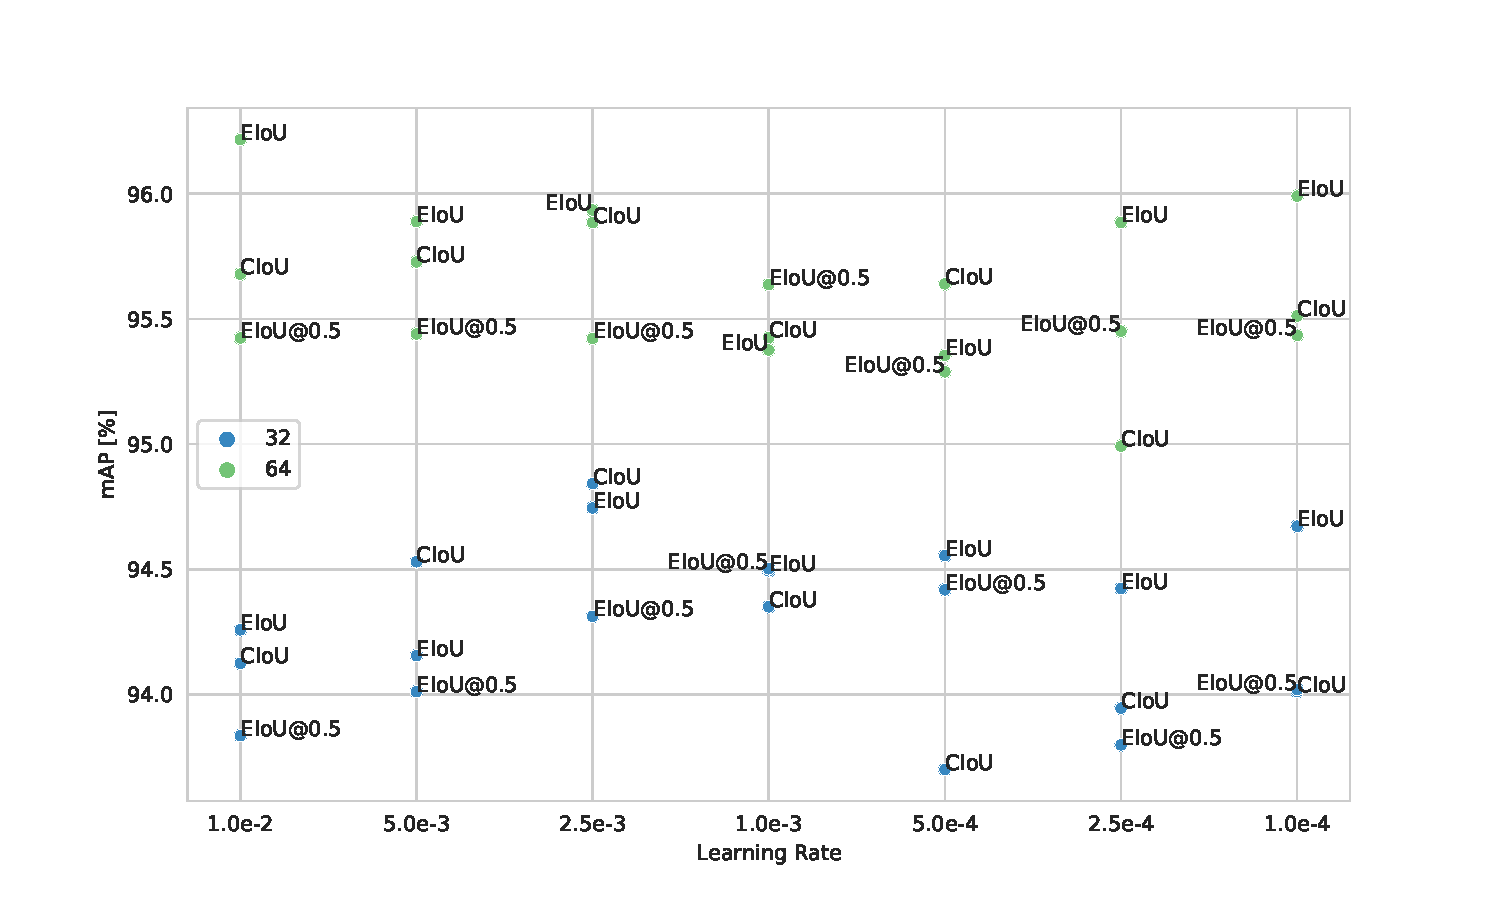
\includegraphics[width=12cm]{imgs/yolo_grid_bs_compare.pdf}
    \caption{Results of the grid search shown for all loss functions, learning rates and batch sizes.}
    \label{fig:yolo_grid_bs_compare_results}
\end{center}
\end{figure}

Figure \ref{fig:yolo_grid_heat_results} shows a heat map for all possible configurations trained with a batch size of 64.
It can be observed that networks trained with \ac{EIoU} performed better over all learning rates, while those trained with \ac{CIoU} performed second best and networks trained with Focal-\ac{EIoU} performed the worst.
For fine tuning of the thresholds used in during the training the best performing network from the grid search is selected.

\begin{figure}
\begin{center}
    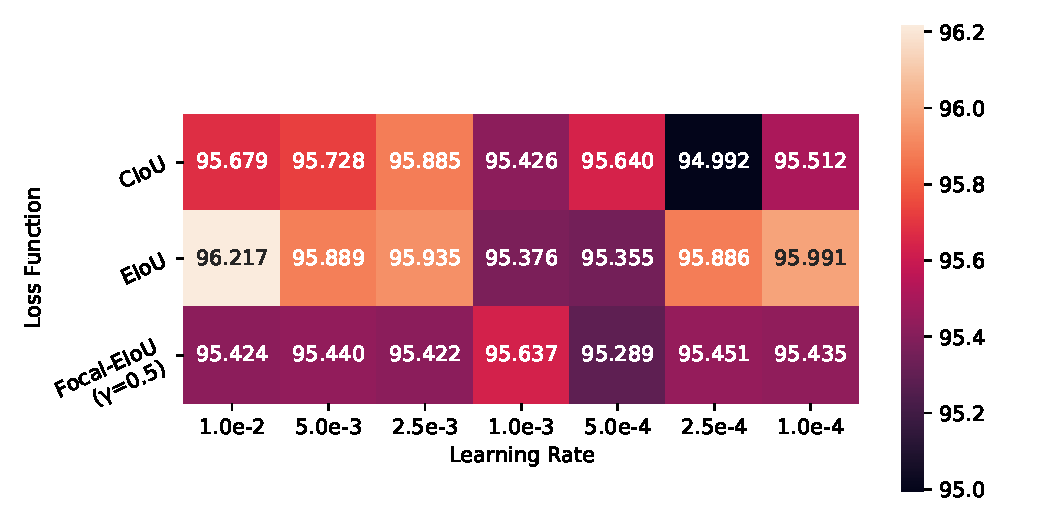
\includegraphics[width=16cm]{imgs/yolo_grid_heat.pdf}
    \caption{Results of the YOLO grid search for all used loss functions and learning rates shown for batch size 64.}
    \label{fig:yolo_grid_heat_results}
\end{center}
\end{figure}

\subsubsection{Tuning: Input Size}

Redmon et al. \cite{yolov2} normally trained their YOLO networks with a small input resolution and after training increased it to get a further boost in performance.
The same is done in this thesis.
The networks were trained with an input size of $608 \times 608$, which is the default input size for \ac{YOLOv4}-Tiny.
The new input size was tuned on the validation set, for each tested input size the \ac{mAP} was recorded and the results can be seen in figure \ref{fig:yolo_input_size}.
The input size $736 \times 736$, shows an increase in performance and is hence selected for further tuning.

\begin{figure}
\begin{center}
    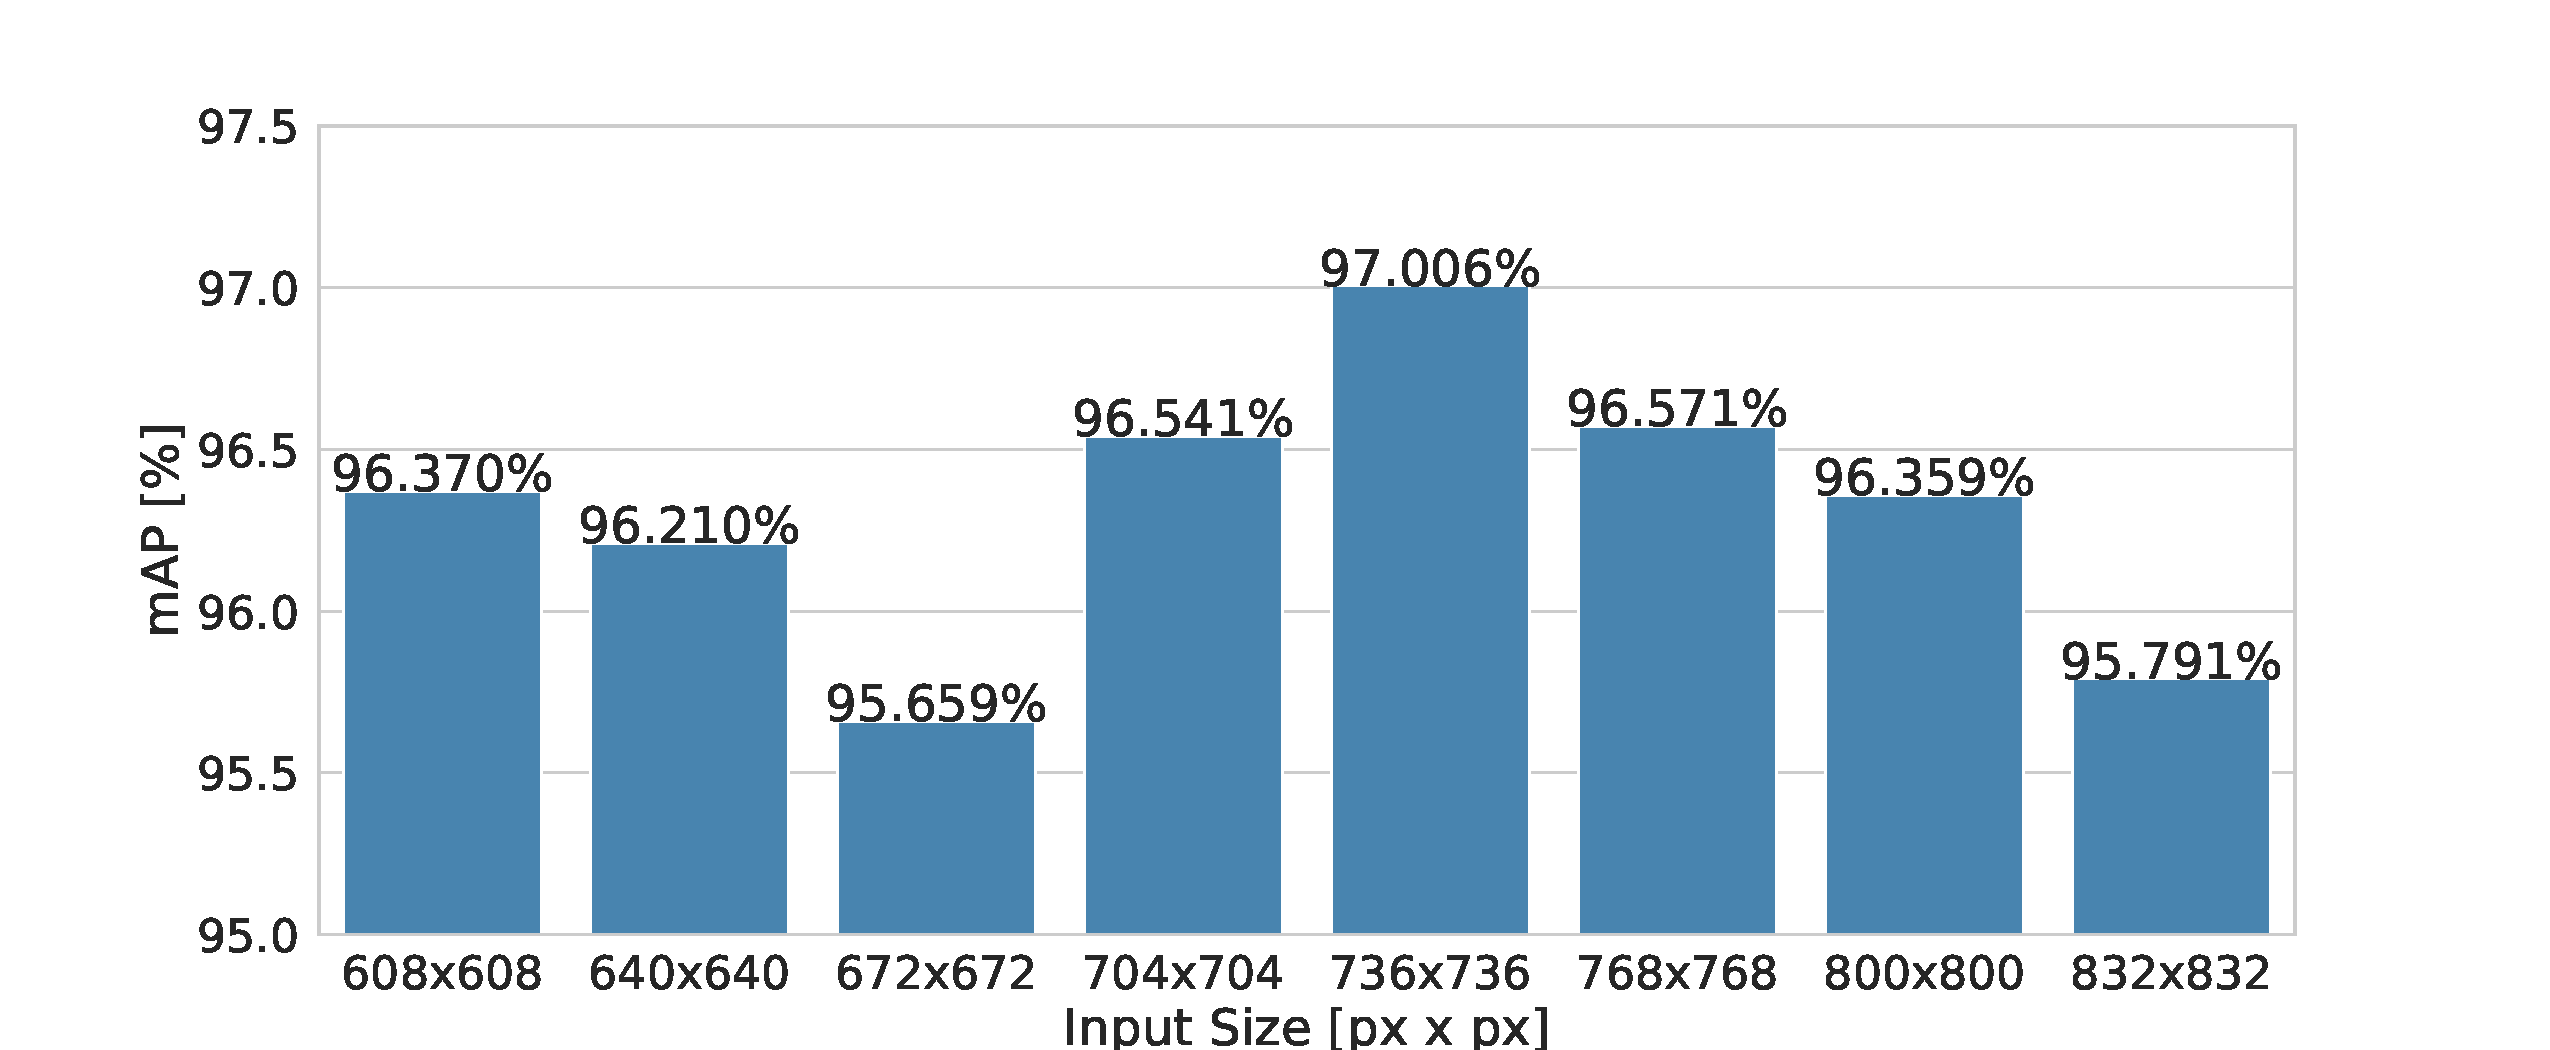
\includegraphics[width=14cm]{imgs/yolo_input_size_tuning.pdf}
    \caption{Different input sizes tested after training on the validation set. The scalar on the x-axis should be interpreted as $val \times val$, since the input size is quadratic.}
    \label{fig:yolo_input_size}
\end{center}
\end{figure}

\subsubsection{Experiment: Non-Maximum Suppression and Test-Time Augmentation}

YOLO predicts multiple bounding boxes per object.
To suppress unnecessary ones and keep only the most suitable, \ac{NMS} is used.
The used \ac{NMS} algorithm during all previous experiments was \ac{DIoU}-\ac{NMS} \cite{diou}.
In this subsection the results are also evaluated using the \ac{WBF} algorithm \cite{weighted_bbox_fusion}, which has shown to perform well in combination with \ac{TTA}.
Both algorithms were explained in section \ref{sec:yolo}.
All tunings are performed only on the validation dataset, with the new input size of $736 \times 736$.

First a tuning of the \ac{DIoU}-\ac{NMS} thresholds is performed.
To recall, \ac{DIoU}-\ac{NMS} takes as input two thresholds a score threshold, which will remove predictions with a prediction score below that one, and an \ac{IoU} threshold which is used to define whether two bounding boxes are the same one, i.e. if two bounding boxes have an $IoU > IoU_{thresh}$, then only the one with the maximum prediction score is kept and the other one is removed.
The tuning was performed on all possible combinations of score threshold and \ac{IoU} threshold, where both have the same parameter set.
The parameter set for both is ranging from 0.1 to 0.5 in 0.05 steps.
The results of the tuning can be found in figure \ref{fig:diou_nms_tuning}.
The best performing combination has a score threshold of 0.1 and a \ac{IoU} threshold of 0.45.

\begin{figure}
\begin{center}
    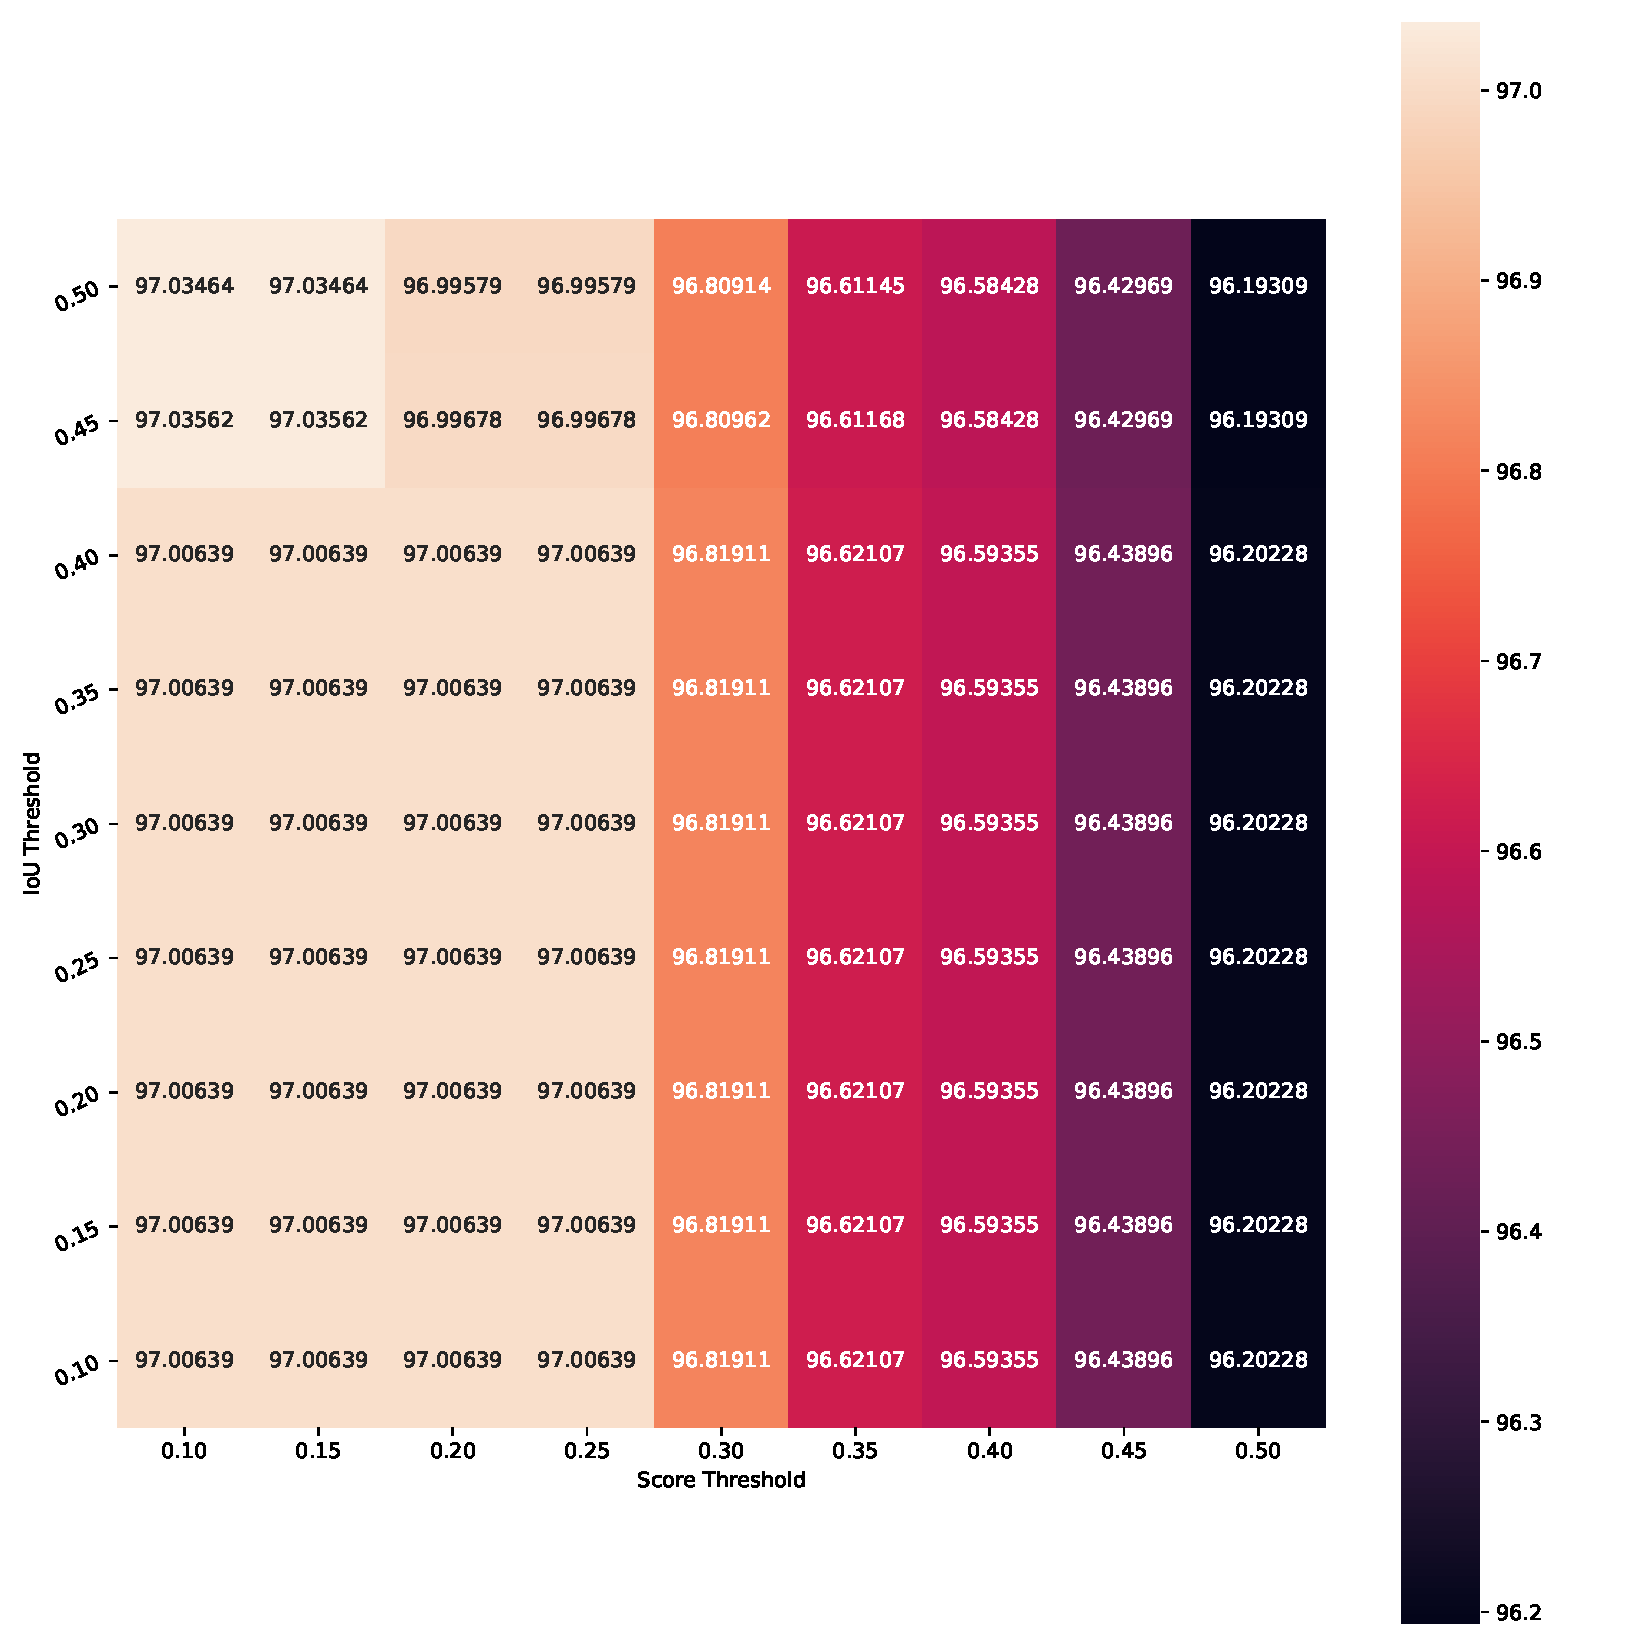
\includegraphics[width=\columnwidth]{imgs/yolo_diou_heat.pdf}
    \caption{The results of the \ac{DIoU}-\ac{NMS} parameter tuning. All possible combinations of score threshold and \ac{IoU} threshold were evaluated on the validation set. The best performing combination is the one with a score threshold of 0.1 and a \ac{IoU} threshold of 0.45.}
    \label{fig:diou_nms_tuning}
\end{center}
\end{figure}

The second tuning is done using the above setup, except that now the thresholds are tuned for the \ac{WBF} algorithm.
The results the tuning are shown in figure \ref{fig:wbf_nms_tuning}.
The best performing configuration has a score threshold of 0.15 and an \ac{IoU} threshold of 0.25.
Further, \ac{WBF} shows slightly better results with a relative improvement of 0.15\%.
This improvement was expected, since in the predictions with the DIoU-NMS, some \acp{FP} were found, where multiple bounding boxes were predicted for the same text object.
In \ac{WBF} such predictions are fused into one bounding box, hence the slight increase in performance.

\begin{figure}
\begin{center}
    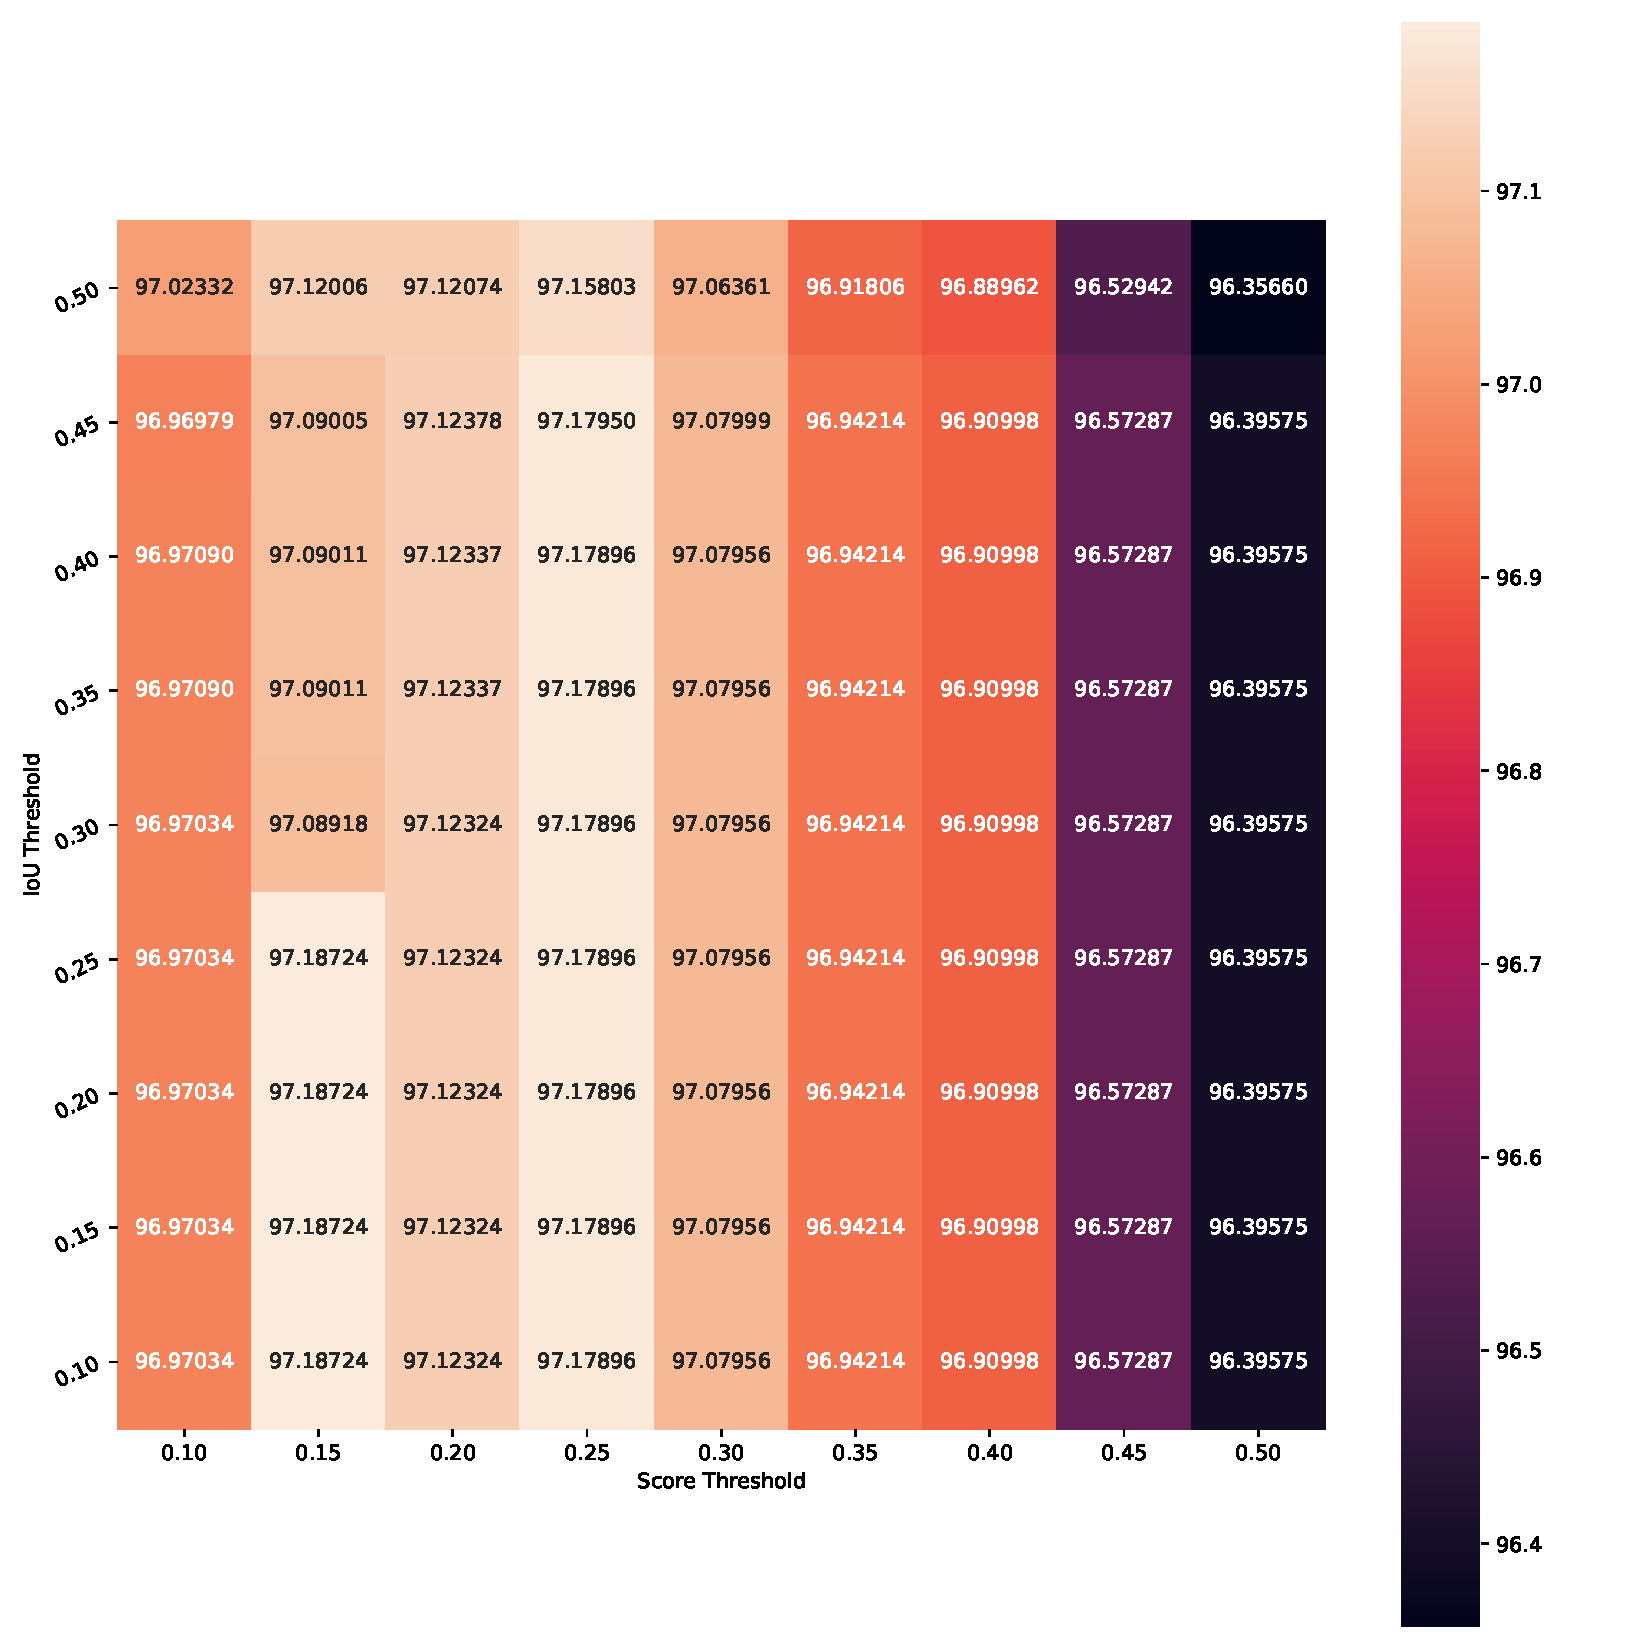
\includegraphics[width=\columnwidth]{imgs/yolo_wbf_heat.pdf}
    \caption{The results of the \ac{WBF} parameter tuning. All possible combinations of score threshold and \ac{IoU} threshold were evaluated on the validation set. The best performing combination is the one with a score threshold of 0.15 and an \ac{IoU} threshold of 0.25.}
    \label{fig:wbf_nms_tuning}
\end{center}
\end{figure}

In the last tuning additionally \ac{TTA} is added to the configuration.
The used augmentations are, as in the offline augmentation experiment, three 90\textdegree\ rotations of the original image, a horizontal flip and again three 90\textdegree\ rotations of the horizontally flipped image.
This experiment also uses \ac{WBF} to merge the predicted bounding boxes.
The full results of this tuning can be found in figure \ref{fig:wbf_tta_nms_tuning}, where the best configuration has a score threshold of 0.1 and an \ac{IoU} threshold of 0.45.
The relative improvement of \ac{WBF}-\ac{TTA}, compared to \ac{DIoU}-\ac{NMS} is 1.5\%.
For the sake of completeness it should be noted that, \ac{TTA} was also performed in the combination with \ac{DIoU}-\ac{NMS}, but this actually slightly worsened the results, when comparing them to \ac{DIoU} without \ac{TTA}.

% \begin{figure}
% \begin{center}
%     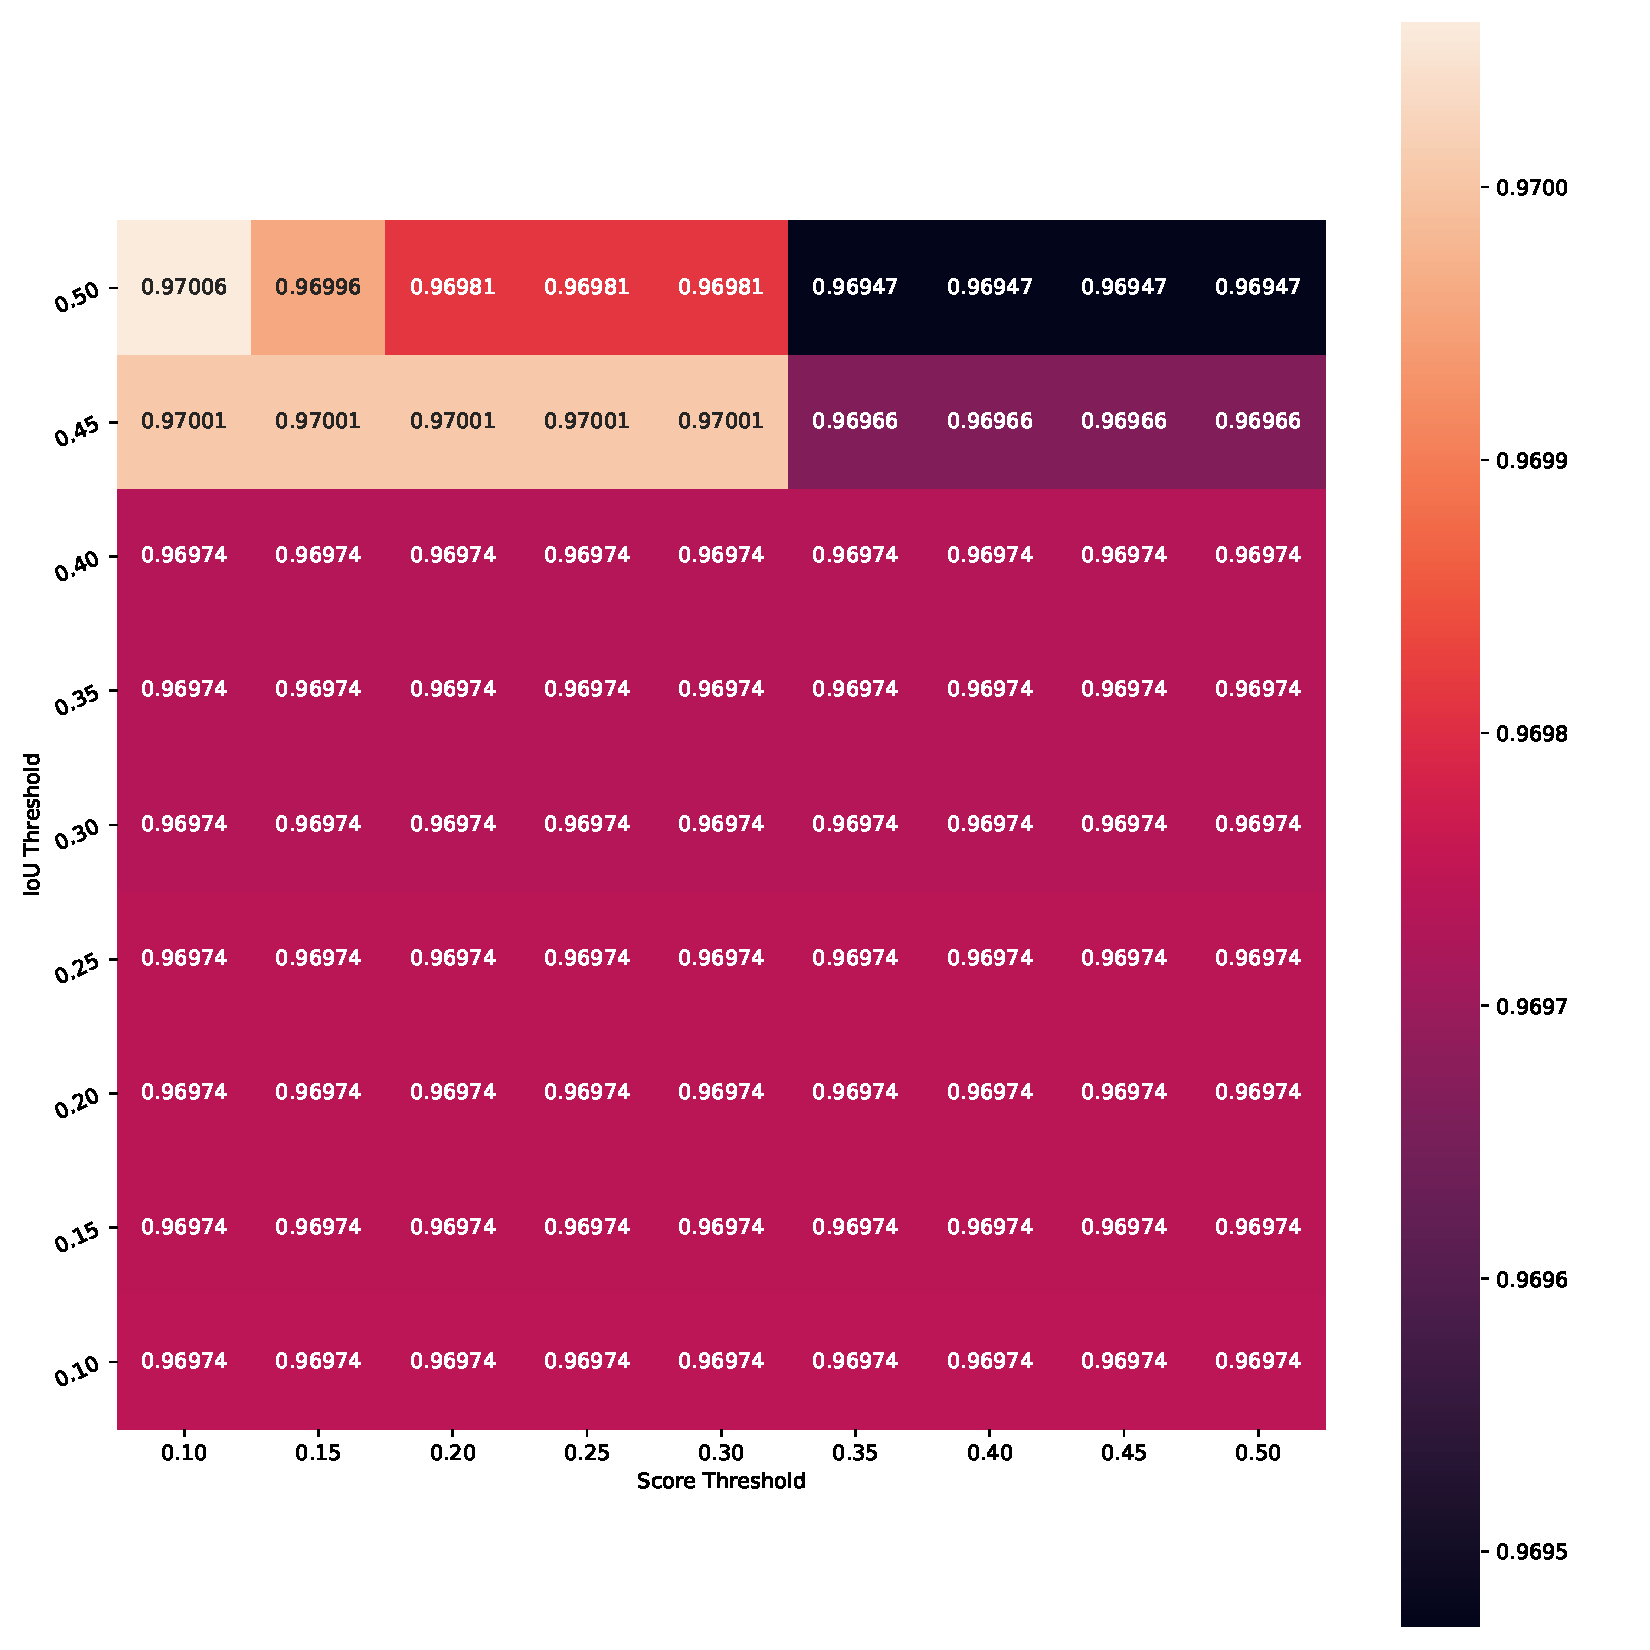
\includegraphics[width=\columnwidth]{imgs/yolo_diou_tta_heat.pdf}
%     \caption{DIOU + TTA TUNING}
%     \label{fig:diou_tta_nms_tuning}
% \end{center}
% \end{figure}

\begin{figure}
\begin{center}
    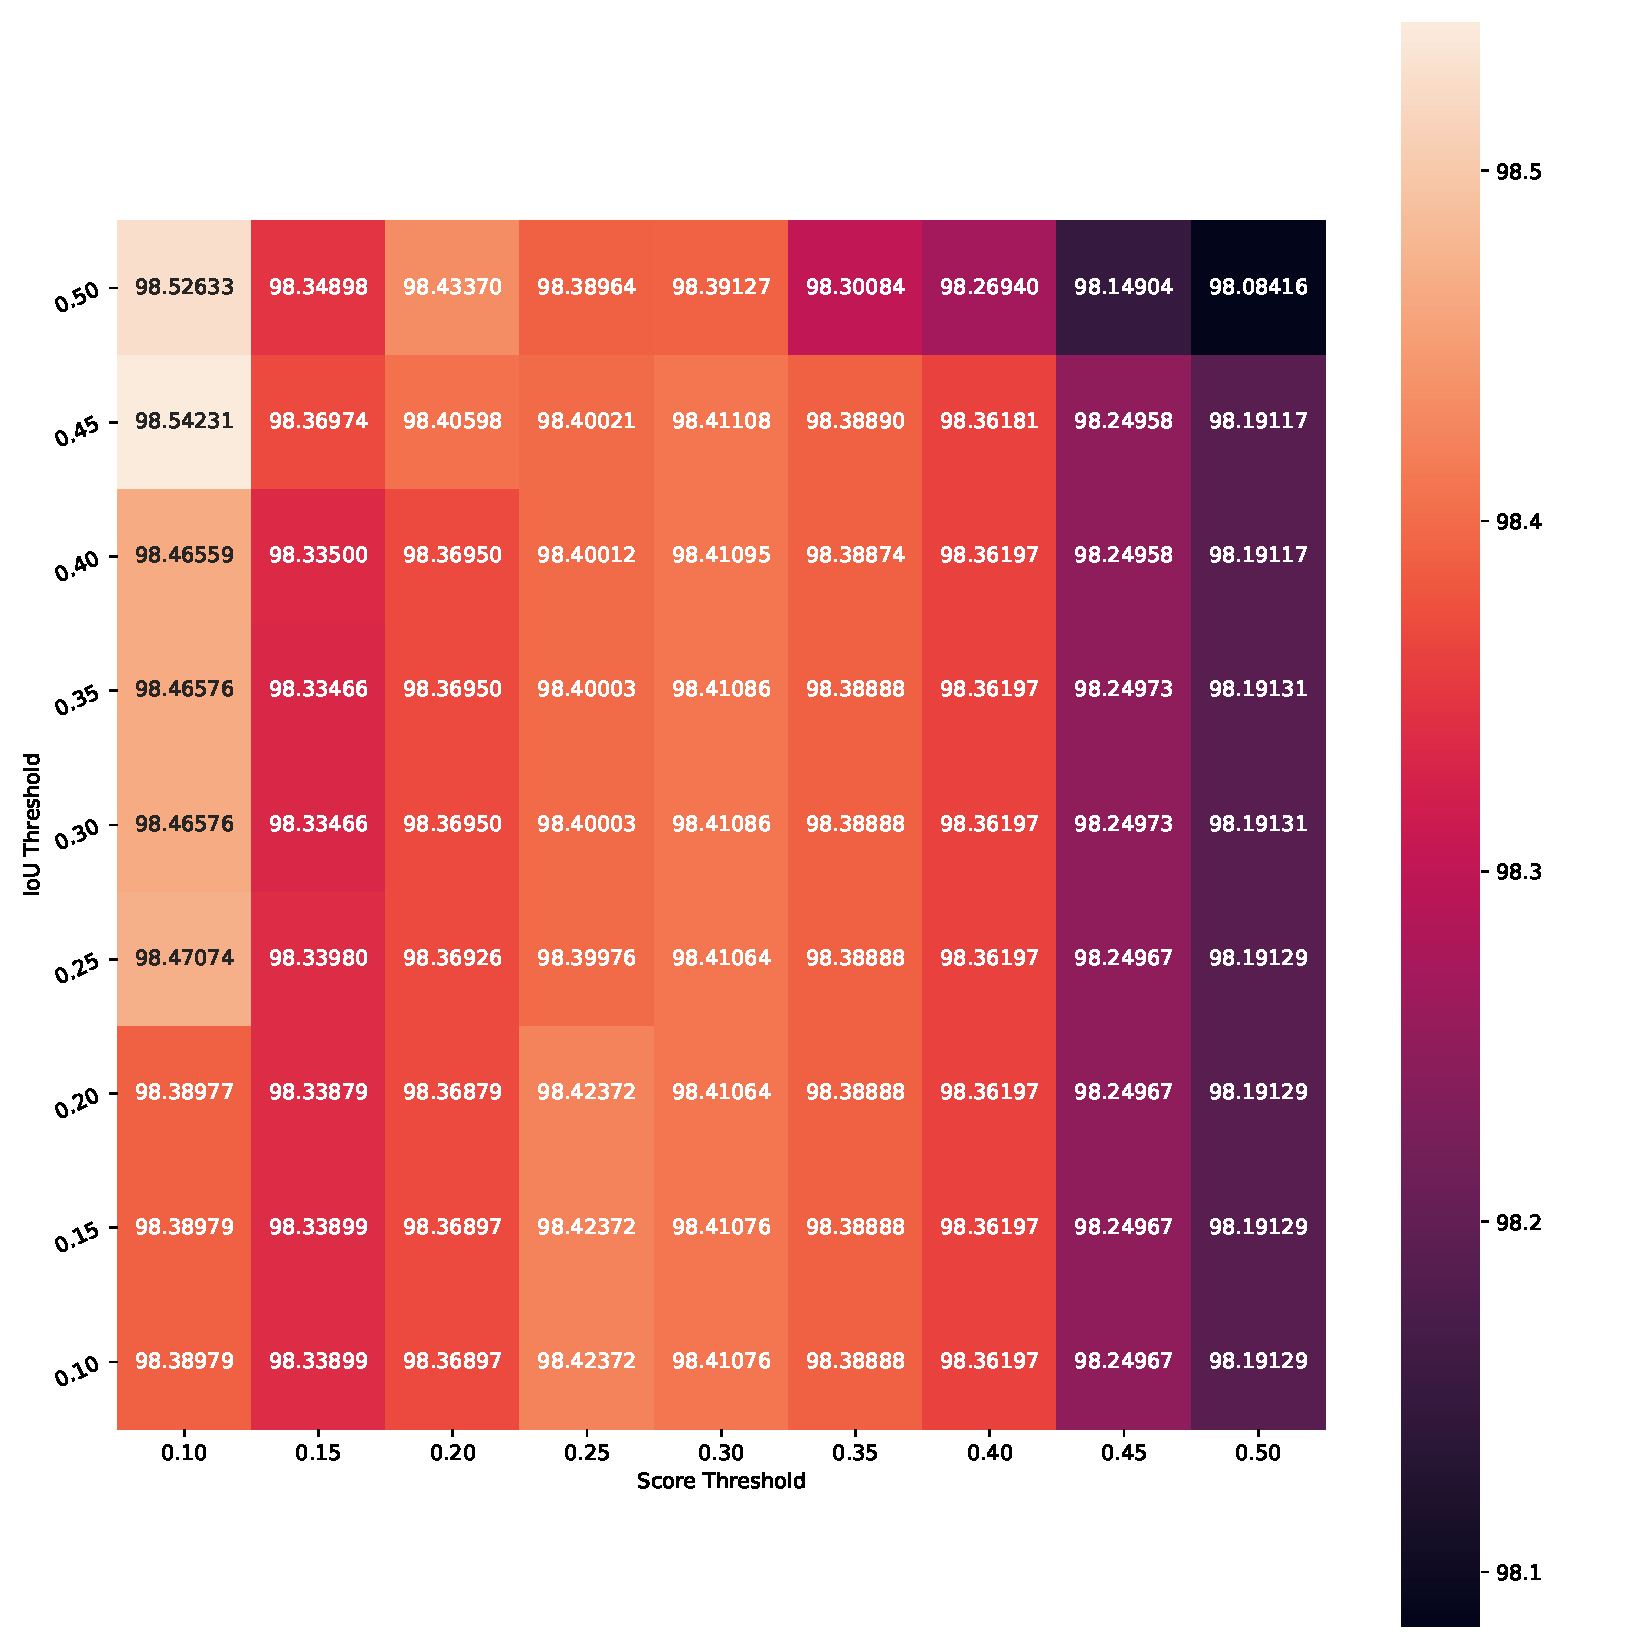
\includegraphics[width=\columnwidth]{imgs/yolo_wbf_tta_heat.pdf}
    \caption{WBF + TTA TUNING}
    \label{fig:wbf_tta_nms_tuning}
\end{center}
\end{figure}


\begin{figure}
\begin{center}
    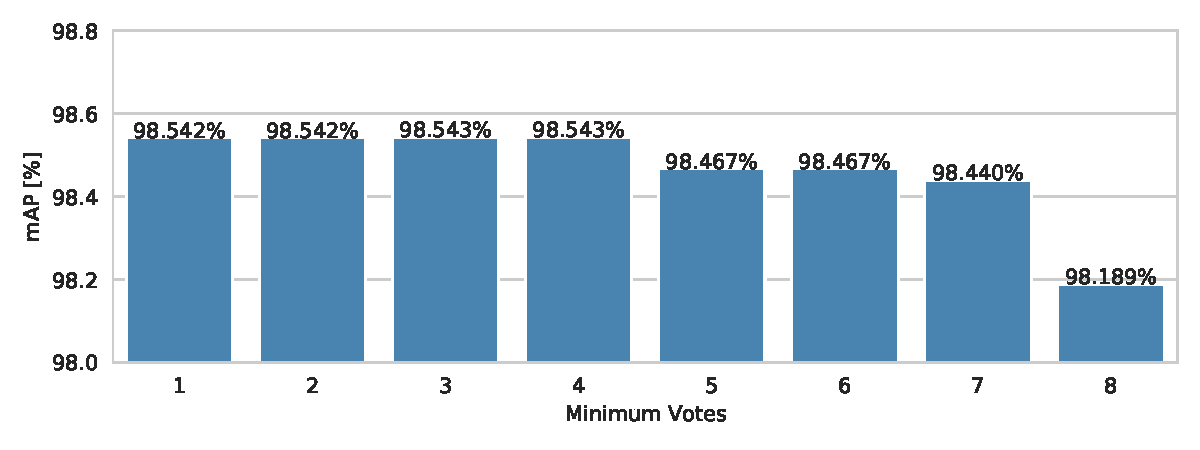
\includegraphics[width=\columnwidth]{imgs/yolo_wbf_tta_votes.pdf}
    \caption{WBF + TTA + VOTES}
    \label{fig:wbf_tta_nms_votes}
\end{center}
\end{figure}


\begin{figure}
\begin{center}
    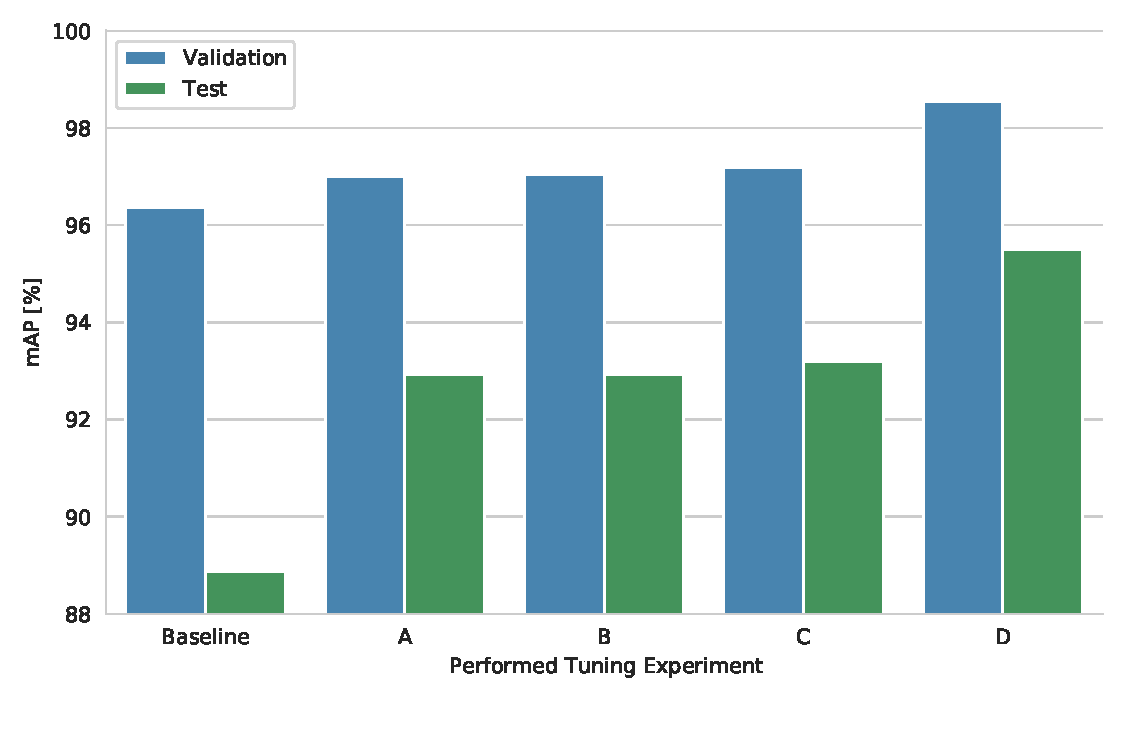
\includegraphics[width=\columnwidth]{imgs/yolo_all_tuning.pdf}
    \caption{Combined tuning results}
    \label{fig:yolo_tuning_combined_results}
\end{center}
\end{figure}

% \subsection{MobileNetV2-UNet}




% \subsubsection{Experiment: Initial Learning Rate Search}

% \subsubsection{Experiment: Offline Augmentations}

% \subsubsection{Experiment: Online Augmentations}

% \subsubsection{Experiment: Grid Search}

% \subsection{MobileNetV2-UNet}
